\section{Research Method}

We adopted Grounded Theory (GT) as research method. GT is a method originally
proposed in \cite{glase1967discovery} which has as distinguishing features the
absence of clear research hypothesis upfront and limitation of literature
exposure at the beginning of the research. Is a theory-developing approach in
contrast with the more traditional theory-testing approach
\cite{coleman2007using}.

Some of related work claimed to used "GT inspired" approaches. It is a very
common rhetoric in recent research on software engineering, but only research
that embodies GT’s core principles should claim to be a grounded theory study
\cite{stol2016grounded}.

GT was employed as the research method for the following reasons:
\begin{itemize}

\item GT is a consolidated method in other areas of research like sociology,
nursing, education and finances and is increasingly being employed
to study software engineering topics \cite{stol2016grounded};

\item GT is considered an adequate approach to investigate scenarios with
questions such as \textit{what's going on here?} \cite{barnsteiner2002using},
which is exactly the scenario proposed here, what's going on DevOps adoption?

\item GT allows the researcher to get descriptions without bias of previous
researches, which is adequate to collect empirical evidence directly from the
practice on industry. The evidence is only reintegrated back with literature
after the theory construction.

\end{itemize}

Since the publication of the original version in \cite{glase1967discovery},
several modifications and variations occurred in the original text, coming to
exist at least seven different versions of the method \cite{denzin2007grounded},
where the main versions are those of Glaser or classic, Strauss and
Charmaz \cite{stol2016grounded}. The study presented in \cite{stol2016grounded}
explores the main aspects of GT versions and establishes that GT studies has to
specify which version is used on it. In our study, we choose the classic
version. The first reason to our choice is that we did not have a research
question at the beginning of the research, exactly as suggested in the classic
version, we start from a interest area that are: successfully DevOps adoption
in industry. And the second reason is because the more detailed papers in
software engineering research use predominantly this version
\cite{stol2016grounded}.

\subsection{GT Procedures}

In Fig. \ref{fig1}, reproduced from \cite{adolph2011using}, is showed the view
of the grounded theory procedures that we followed in the conduction of this
research.

\begin{figure}[htpb]
  \centering
  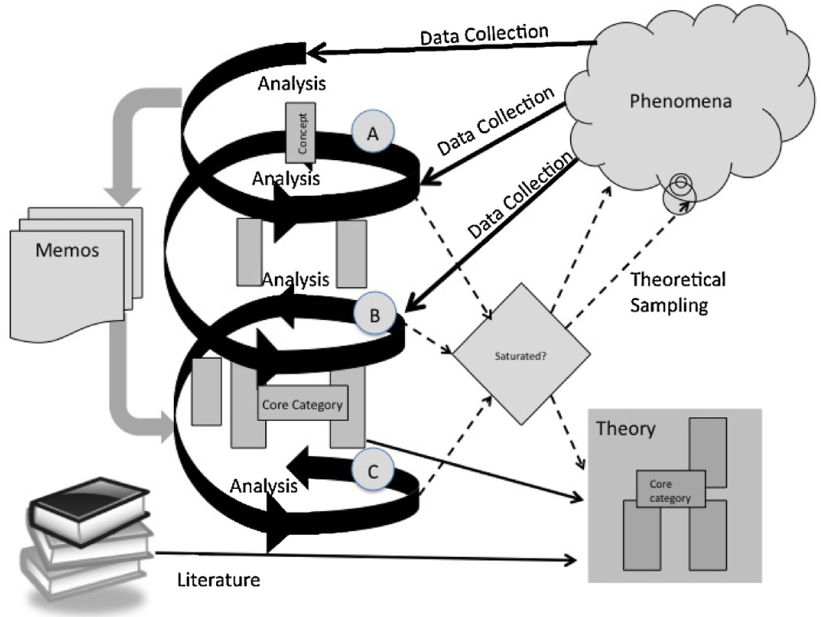
\includegraphics[width=0.5\textwidth,natwidth=821,natheight=617]{GT.png}
  \caption{The GT Method \cite{adolph2011using}}
  \label{fig1}
\end{figure}

\begin{enumerate}[label=(\Alph*)]
\item Initially, we begin collecting data about the adoption process from
companies that have successfully adopted it. As the data were collected, they
were also analyzed simultaneously. The raw data is analysed by searching for
atterns of incidents to indicate concepts, and concepts groupeds into
categories. This first step, where all raw data is analysed, is called open
coding \cite{stol2016grounded}.

\item The categories are developed by constant comparison of new incidents with
previous. Every grounded theory study has to identify a "core category"
\cite{stol2016grounded}. The core category is responsible for enabling the
integration of the other categories and structuring the results into a dense
and consolidated grounded theory \cite{jantunen2014using}. The identification
of the core category represents the end of open coding and the beginning of the
selective coding. In selective coding, only specific variables that are
directly related to the core category and their relationships are coded, in
order to enable the production of a harmonic theory \cite{coleman2007using}
\cite{hoda2011impact}.

\item After saturation, the resulting theory is reintegrated back into
literature comparing with existing theories. The literature search is performed
only later to avoid forcing pre-conceived concepts on the theory development
\cite{adolph2012reconciling}.

\item Throughout the process, memos are writed capturing thoughts and analytic
processes; the memos support the emerging concepts, categories, and their
relationships \cite{adolph2012reconciling}.

\end{enumerate}
